\documentclass{article}

\usepackage[utf8]{inputenc}
\usepackage[german]{babel}
\usepackage{amsmath}
\usepackage{mathtools}
\usepackage{listings}
\usepackage{color}

\usepackage{lstlang0}

\lstdefinestyle{customstyle}{
    backgroundcolor=\color[rgb]{.95,.95,.95},
    basicstyle=\small\ttfamily,
    keywordstyle=\bf\ttfamily\color[rgb]{0,.3,.7},
    commentstyle=\color[rgb]{0.133,0.545,0.133},
    stringstyle={\color[rgb]{0.75,0.49,0.07}},
    numbers=left,
    numbersep=5pt,
    numberstyle=\color[rgb]{0.6,0.6,0.6},
    tabsize=4
}

\begin{document}

\tableofcontents

\section{Geschichte und Einführung}

\subsection{Geschichte}

\begin{enumerate}
    \item Lambda Kalkül
        \begin{itemize}
            \item Gleichwertig mit Turing Maschine (kann gleichen Probleme lösen)
            \item Universale Turing Maschine (kann alle Turingmaschinen beschreiben)
            \item Universale Lambda-Funktion gesucht
        \end{itemize}

    \item Fortran (Fortran list processing language)

    \item Fortran M-Expressions (Idee wurde nie implementiert)

    \item Lisp
        \begin{itemize}
            \item List processing Alternative zu Turingmaschine: LISP Funktion eval
            \item Notation: Programme und Daten können beide als Liste beschrieben werden
                \begin{figure}[h!]
                	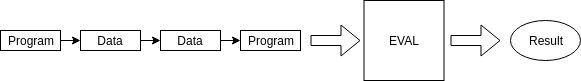
\includegraphics[width=\linewidth]{pics/lisp-notation}
                	\caption{LISP EVAL vereinfacht}
                \end{figure}
            \item EVAL ist LISP Interpreter
        \end{itemize}

    \item Scheme
        \begin{itemize}
            \item Prototyp für funktionale Programmiersprache
            \item Versuch, LISP simpler umzusetzen
            \item Optimized tail recursion (garantiert vom Compiler)
        \end{itemize}
\end{enumerate}

\subsection{Tail call optimization}
Tailcall Rekursion ist fast so effizient wie \textbf{goto} Begehle weil keine neuen
Stackframes aufgebaut werden müssen.

\subsubsection{Tail recursion}
Rekursive Funktion f ist \textbf{endrekursiv}, wenn der rekursive Funktionsaufruf die \textbf{letzte Aktion zur Berechnung von f} ist.

\subsubsection{Beispiele}
\lstset{language=C,style=customstyle}
\begin{lstlisting}
// Kein tail call
int fact(int x){
    if(x == 0) return 1;
    else return fact(x - 1) * x;
}
\end{lstlisting}


\lstset{language=C,style=customstyle}
\begin{lstlisting}
// Tail call
int fact(int x, int accum=1){
    if(x == 0) return accum;
    else return fact(x - 1, x * accum);
}
\end{lstlisting}
\textbf{\textit{Optimierung möglich, da x nicht als Zwischenergebnis gespeichert werden muss.}}


\section{Closures}

\subsection{Static und Dynamic Scoping}
\begin{itemize}
    \item Static/Lexical Scoping: \\
          Struktur des Sourcecodes legt fest welche Variablen gemeint sind.
    \item Dynamic Scoping: \\
          Stack/Programmzustand legt Variablen fest.
\end{itemize}

\subsection{Closure}
Jede Scheme-Funktion hat eigene Umbebung für alle Variablen,
die im body vorkommen. \\\\
\textbf{Closure = Code + Umgebung}

\subsubsection{Beispiel}
\lstset{language=Scheme,style=customstyle}
\begin{lstlisting}
define (new-account)        ;; funktion ohne argumente
    (let ((balance 0))     ;; lokale variable = 0
    (lambda (x)            ;; Rückgabe = Funktion erhöht balance um x und gibt balance zurpck
        (set! balance (+ balance x))
        balance)))

(define ferien (new-account))
(ferien 10)            ;; -> 10
(ferien 10)            ;; -> 20

(define reisen (new-account))
(reisen 3)             ;; -> 3
(ferien 10)            ;; -> 30
\end{lstlisting}


\section{Lambda Kalkül}

\subsection{Bestandteile}
\begin{itemize}
    \item \textbf{Term} \textit{(Kodierte Werte und Funktionen)}
    \item \textbf{Variable}
    \item \textbf{Funktion}
    \item $\lambda$\textbf{-Abstraktion}
\end{itemize}

\subsection{Terme}
\begin{itemize}
    \item Eine Variable ist ein Term
    \item Sind \textbf{t} und \textbf{s} Terme, so ist \textbf{ts} ein Term
          \textbf{\textit{(wird auch Anwendung genannt)}}.
    \item Ist \textbf{t} ein Term und \textbf{x} eine Variable,
          dann ist $\lambda x.t$ eine Abstraktion
\end{itemize}

\subsection{Notation}
\begin{itemize}
    \item Linksklammerung: $xxx = (xx)x$
          \textit{(Rechtsklammerung muss explizit sein)}
    \item Abstraktion mit mehreren Variablen:
          $\lambda x.\lambda y.\lambda z.t = \lambda xyz.t$
\end{itemize}


\section{Gleicheit}

\subsection{Gebundene Variablen}
\begin{itemize}
    \item Alle nicht freien Variablen
    \item können umbennant werden \\
          \textbf{(Solange dadurch keine freien Variablen eingefangen werden)}
\end{itemize}

\subsubsection{Beispiel}
\lstset{language=C,style=customstyle}
\begin{lstlisting}
inline int f(int x){
  int i;
  for(i = 0; i < 10; i++) x=x*x;
  return x
}

int main(){
  int x; int i; x=3; i=6;
  f(x); f(i); f(5);
  return 0;
}
\end{lstlisting}

\subsubsection{Freie Variablen}
Variable x in Term t is freie Variable wenn $x \in FV(t)$ \\
\textbf{Eine Variable ist element von FV wenn:}
\begin{itemize}
    \item t eine Variable x ist: \textbf{FV(t) = {x}}
    \item t eine Anwendung vs ist: \textbf{FV(t) = FV(v) $\cap$ FV(s)}
    \item t eine Abstraktion $\lambda x.s$ ist: \textbf{FV(t) = FV(s)\textbackslash{x}}
\end{itemize}

\subsection{Einsetzen in Terme}
Einsetzen eines Terms s in einen Term t für die Variable x: \textbf{t[x$\leftarrow$s]}

\subsubsection{Regeln}
\begin{itemize}
    \item t ist Variable
    \begin{enumerate}
        \item $t=x$; $x[x\leftarrow s]=s$
        \item $t=y$; $y[x\leftarrow s]=y$ \textit{nicht-x-Variable wird nicht ersetzt}
    \end{enumerate}
    \item t ist Anwendung pq
    \begin{enumerate}
        \item $t=pq$; $pq[x\leftarrow s]=p[x\leftarrow s] q[x\leftarrow s]$
    \end{enumerate}
    \item t ist Abstraktion
    \begin{enumerate}
        \item $t=\lambda x.r$; $\lambda x.r[x\leftarrow s]=\lambda x.r$
        \item $t=\lambda y.r$; $y\neq x$
        \begin{itemize}
            \item $y \notin FV(s) \implies \lambda y.r[x\leftarrow s]=\lambda y.(r[x\leftarrow s])$
            \item $y \in FV(s) \implies$ Umbenennung der gebundenen Variable:\\
                  $\lambda y.r = \lambda z.r[y\leftarrow z] \implies (\lambda z.r[y\leftarrow z])[x\leftarrow s]$
        \end{itemize}
    \end{enumerate}
\end{itemize}

\subsubsection{Beispiele}
\begin{itemize}
    \item $x[x\leftarrow \lambda z.z] = \lambda z.z$
    \item $yy[x<-\lambda z.z] = yy$
    \item $(\lambda z.xy)[x\leftarrow y] = \lambda z.yy$
    \item $(\lambda z.xy)[x\leftarrow z] = \lambda p.(xy[z\leftarrow p])[x\leftarrow z] = \lambda p.zy$
\end{itemize}

\subsection{\alpha -Gleicheit}
$\lambda x.t = \lambda y.(t[x\leftarrow y])$ \textit{(falls y nicht in FV(t))}

\subsection{\beta -Gleicheit}
$(\lambda x.t)s = t[x\leftarrow s]$

\subsection{\eta -Gleicheit}
$(\lambda x.tx) = t$ \textit{(falls x nicht in FV(t))}


\section{Makros}

\subsection{Booleans und If}
\begin{itemize}
    \item true: \lambda xy.x
    \item false: \lambda xy.y
    \item if: \lambda xyz.xyz
    \item not: \lambda x.if x false true
    \item and: \lambda xy.if x y false
\end{itemize}

\subsection{Zahlen (Church Nummerals)}
\begin{itemize}
    \item 0 = \lambda fx.x
    \item 1 = \lambda fx.fx
    \item 2 = \lambda fx.f(fx)
    \item n = $\lambda fx.f^nx$
\end{itemize}

\subsubsection{Addition}
\lambda mn.\lambda fx.mf(nfx)

\subsubsection{Multiplikation}
\lambda mn.\lambda fx.m(nf)x

\subsection{Listen}
\begin{itemize}
    \item cons: \lambda abc.if c a b
    \item car: \lambda p.p true
    \item cdr: \lambda p.p false
\end{itemize}

\subsection{For loop}
n f \textit{(n = Church Numeral)}


\section{Rekursion}

\subsection{Primitive Rekursion}
Kann in endlichen Schritten gelöst werden: \\
\textbf{if, for, listen, etc...}

\subsection{Allgemeine Rekursion}
Nicht ohne Fixpunktoperator möglich

\subsubsection{Fixpunktoperator (Y-Combinator)}
\begin{itemize}
    \item \textbf{Fixpunkt:} f = \lambda x.if (< x 2) 1 (+ (f (- x 1)) (f (- x 2)))
    \item \textbf{Rekursion:} F = \lambda fx.if (< x 2) 1 (+ (f (- x 1)) (f (- x 2)))
    \item f = F f \textit{(f ist ein Fixpunkt von F)}
\end{itemize}

Für ein beliebiges \textbf{F} ist \textbf{YF} ein Fixpunkt:
Y = \lambda g.(\lambda x.g(xx)) (\lambda x.g(xx))

\begin{enumerate}
    \item YF = \lambda (g.(\lambda x.g(xx))(\lambda x.g(xx))) F
    \item (\lambda x.F(xx))(\lambda x.F(xx))
    \item F((\lambda x.F(xx)) (\lambda x.F(xx)))
    \item F((\lambda g.(\lambda x.g(xx)) (\lambda x.g(xx))) F)
\end{enumerate}


\section{Lambda Umgebung}
Ist \textbf{partielle Abbildung der variablen} in die Terme
einer Definitionsmenge \textbf{(Domain)}

\subsection{Spezielle Umgebungen}
\begin{itemize}
    \item \varepsilon ist die \textbf{leere Umgebung}
    \item Umgebungen mit genau einer Variablen sind \textbf{Bindungen}
    \begin{itemize}
        \item Schreibweise: $x \rightarrow t$, $dom(\phi) = {x}$, $\phi(x)=t$
        \item Komposition $\phi \circ \psi$ \textit{(\phi und \psi sind Umgebungen)}:
        \begin{itemize}
            \item $dom(\phi \circ \psi) = dom(\phi) \cup dom(\psi)$
            \item \[(\phi \circ \psi)(x) =
                    \begin{cases}
                        x \in dom(\phi) & \phi(x) \\
                        sonst           & \psi(x)
                    \end{cases}\]
            \item dom(\phi) ist endlich und besteht aus Bindungen $\psi_i$ \\
            $\phi = \psi_0 \circ \psi_1 \circ \psi_2 \cdots \psi_n$
        \end{itemize}
    \end{itemize}
\end{itemize}

\subsection{Auswertung}
Die Auswertung einer Variablen \textbf{t} in \phi wird geschrieben $t \downarrow \phi$

\subsubsection{Regeln}
\begin{enumerate}
    \item Variable x
    \begin{itemize}
        \item $x \downarrow \phi = \phi(x)$
        \item $x \downarrow \phi = x$ \textit{(wenn x $\notin$ dom(\phi))}
    \end{itemize}
    \item Anwendung s auf r \textbf{(rs)} \\
    sei $p = r \downarrow \phi$ und $q = s \downarrow \phi$
    \begin{itemize}
        \item wenn p die Form \lambda x.u hat so ist
        $rs \downarrow \phi = u \downarrow [q \leftarrow x] \circ \phi$
        \item Andernfalls: $rs \downarrow \phi = p \circ q$
    \end{itemize}
    \item Abstraktion \lambda x.s \\
    $\lambda x.s \downarrow \phi = \lambda z.(s \downarrow (z \leftarrow x) \circ \phi)$ \\
    Wobei $z \notin FV(s) \cup \bigcup_{y \in dom(\phi)}FV(\phi(y))$
\end{enumerate}

\subsubsection{Beispiele}
\lstset{language=Scheme,style=customstyle}
\begin{lstlisting}
(let ((a 1))
     (plus10 (let ((a 10))
                  (lambda (x) (+ a x))))
     (let ((y 5) (x 3))
          (plus10 (+ a y))))
\end{lstlisting}
\begin{figure}[h!]
    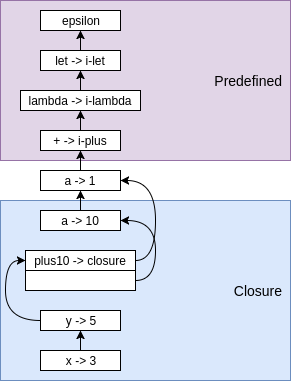
\includegraphics[scale=.5]{pics/i-environment}
    \caption{Lambda Bindings}
\end{figure}


\section{\lambda -Term Auswertung}

\subsection{Beispiele: Umgebung}
\begin{itemize}
    \item $(\lambda x.t) s \downarrow \phi$
    \begin{itemize}
        \item $s \downarrow \phi$
        \item $t \downarrow (s \leftarrow x) \circ \phi$
        \item $x \downarrow \phi = x$ falls $x \notin dom(\phi)$
    \end{itemize}

    \item $(\lambda x.t) \downarrow \phi = \lambda x.(t \downarrow \phi)$
    falls $x \notin \phi(y)$ für alle $y \in dom(y)$.

    \item $\lambda mnfx.mf(nfx)$ und $1 = \lambda gy.gy$
    \begin{enumerate}
        \item $((+ 1) 1) \downarrow \varepsilon$
        \item $1 \downarrow \varepsilon \rightarrow \lambda g.(\lambda y.gy) \downarrow \varepsilon$
        \item $\lambda g.(\lambda y.gy) \downarrow \varepsilon$
        \item $\lambda g.((\lambda y.gy) \downarrow \varepsilon)$
        \item $\lambda g.\lambda y.(gy \downarrow \varepsilon) = \lambda g.\lambda y.(g \downarrow \varepsilon)(y \downarrow \varepsilon) = 1$
        \item $(+ 1) \downarrow \varepsilon$
        \item $\lambda m.(\lambda nfx.mf(nfx)) 1 \downarrow \varepsilon$
        \item $\lambda nfx.(mf(nfx) \downarrow [1\leftarrow m] \circ \varepsilon)$
        \item $\lambda nfx.(m \downarrow [1\leftarrow m] \circ \varepsilon) f(nfx)$
        \item $\lambda nfx.1f(nfx)$
        \item $(+ 1) 1 \downarrow \varepsilon$
    \end{enumerate}
\end{itemize}


\section{Kombinatoren}
Sind Lambdaterme ohne freie Variablen \textit{(geschlossene Terme)}


\end{document}
